\section{改进的U-Net模型设计}

% 总领起始段

\subsection{网络的改进设计}

\subsubsection{网络改进方案概述}

尽管U-Net网络的跳跃连接能够有效地结合浅层和深层特征,但直接将编码器浅层特征映射与对应解码器特征级联,这种“无差别”拼接会把大量与前景无关的背景噪声一并传递,造成解码器在处理边界模糊和极小目标时,可能因为上下文信息的缺失而导致定位不准确。

基于上诉分析,为了抑制冗余背景,同时保持高分辨率的边缘信息,本研究对U-Net的网络结构进行了改进。如图~\ref{fig:attunet_frame}所示,改进后的U-Net网络在每一级跳跃通路中引入了注意力门。

\begin{figure}[htbp]
    \centering
    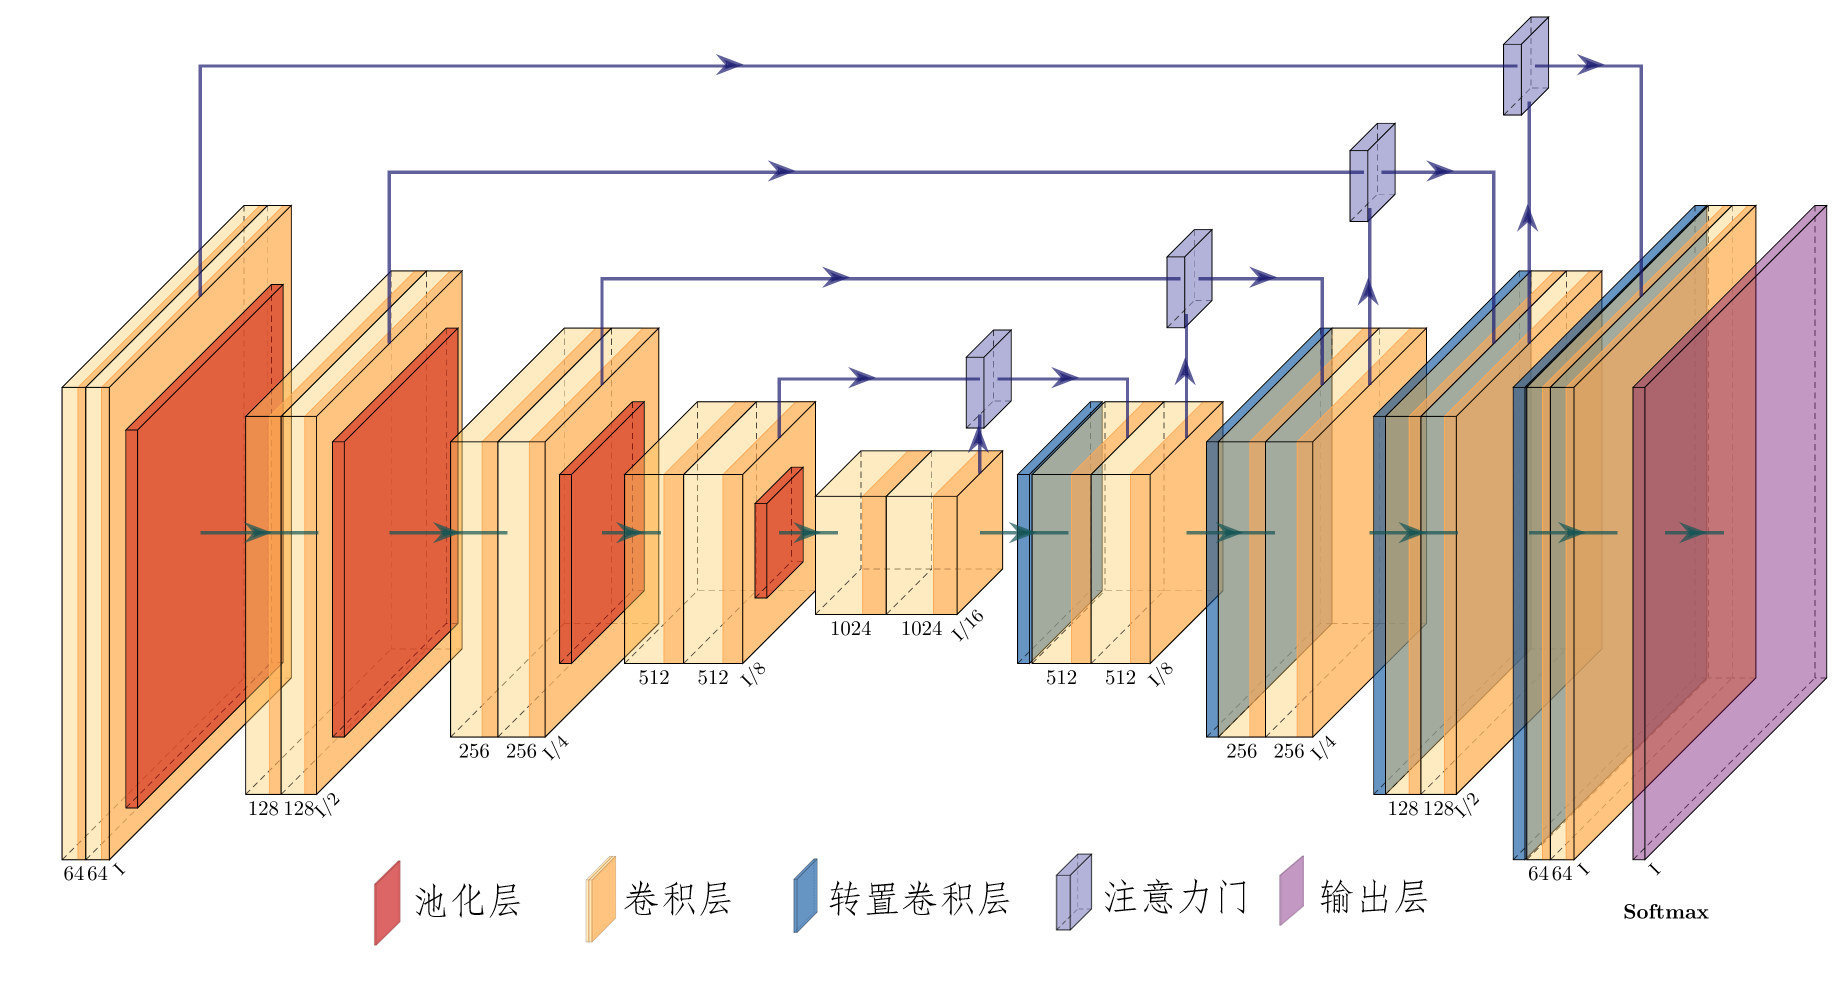
\includegraphics[width=\textwidth]{fig/attunet_frame.png}
    \caption{改进后的U-Net模型网络结构}
    \label{fig:attunet_frame}
\end{figure}

注意力机制的核心要点在于,依靠动态调节特征图的权重,提高模型对于关键区域的敏感程度,减少无关背景带来的干扰,从而提升针对小目标的定位水平\cite{oktay2018}。展开来说,注意力门会依据输入特征图以及从粗尺度提取的上下文信息,计算每个像素的注意力系数,借助此系数对特征图加以加权,仅保留对分割任务有帮助的区域。注意力机制的具体结构和原理在下一节展开叙述。

\subsubsection{注意力门模块的结构与原理}

注意力门模块的内部结构主要由三个关键部分组成:输入特征的加权过程、注意力系数的计算以及门控机制的输出。具体而言,该模块包括权重矩阵 $W_x$ 和 $W_g$、非线性激活函数 ReLU、Sigmoid 激活函数以及注意力权重的计算等组成部分。

首先,注意力门模块接收来自U-Net编码器的特征图 $x_l$ 和解码器的门控信号 $g_l$ 作为输入。$x_l$ 为编码器第 $l$ 层输出的特征图,$g_l$ 则是来自解码器的特征图,它为后续的注意力加权提供上下文信息。为了将这两者的特征进行融合,模块采用了两种1×1卷积操作:一个用于处理编码器的特征图 $x_l$,另一个用于处理解码器的门控信号 $g_l$。这两者都通过对应的卷积核 $W_x$ 和 $W_g$ 进行映射到一个中间空间,从而保持信息的一致性并准备后续的注意力计算。

接下来,在这两路特征图被处理后,它们通过ReLU激活函数进行非线性转换,这一步骤有助于引入非线性特征表达,使得网络能够更好地学习到复杂的关系。此时,经过ReLU激活的特征图被送入一个加法操作,进行特征融合,得到一个结合了编码器和解码器信息的中间表示。为了进一步处理该表示并生成最终的注意力权重,模块通过Sigmoid激活函数计算得到一个归一化的注意力系数 $\alpha_l$,该系数决定了每个像素的权重。最后,这些权重通过逐元素相乘的方式与编码器特征图 $x_l$ 进行加权,从而生成加权后的特征图 $\tilde{x}_l = \alpha_l \cdot x_l$。

在计算过程中,注意力系数 $\alpha_l$ 的计算公式如下:

\begin{equation}
    q_{\text{att}}^l = \psi^T \left( \sigma_1 (W_x^T x_l + W_g^T g_l + b_g) \right) + b_\psi
\end{equation}

\begin{equation}
    \alpha_l = \sigma_2 \left( q_{\text{att}}^l(x_l, g_l; \Theta_{\text{att}}) \right)
\end{equation}

其中,$\sigma_1$ 和 $\sigma_2$ 分别为 ReLU 和 Sigmoid 激活函数,$W_x$ 和 $W_g$ 是用于特征映射的权重矩阵,$\psi$ 是线性变换矩阵,$b_g$ 和 $b_\psi$ 是偏置项。在这个公式中,$q_{\text{att}}^l$ 是通过加法操作和线性变换后得到的注意力得分,$\alpha_l$ 是最终计算得到的注意力系数。通过Sigmoid激活,$\alpha_l$ 的值范围被限制在$[0, 1]$之间,能够根据不同位置的特征重要性动态调整每个位置的注意力权重。

为了进一步探究注意力门的机制和作用,本文直观展示了同一张 ISIC 图像分别在基准 U-Net 与 Attention-U-Net 四级跳跃通路上的特征图,并截取其中 4 个通道进行并排可视化,如图 \ref{fig:skip_vs_gate_vis} 所示。图中左半四列(Skip:ch0-ch3)对应原始U-Net网络的编码器跳跃连接后准备和解码器拼接的特征图;右半四列(Gate:ch0-ch3)则是 Attention U-Net经过注意力门调制后的准备和解码器拼接的特征图。纵向从上到下依次为四级跳跃连接(Skip1/Gate1-Skip4/Gate4)。

\begin{figure}[!htbp]
    \centering
    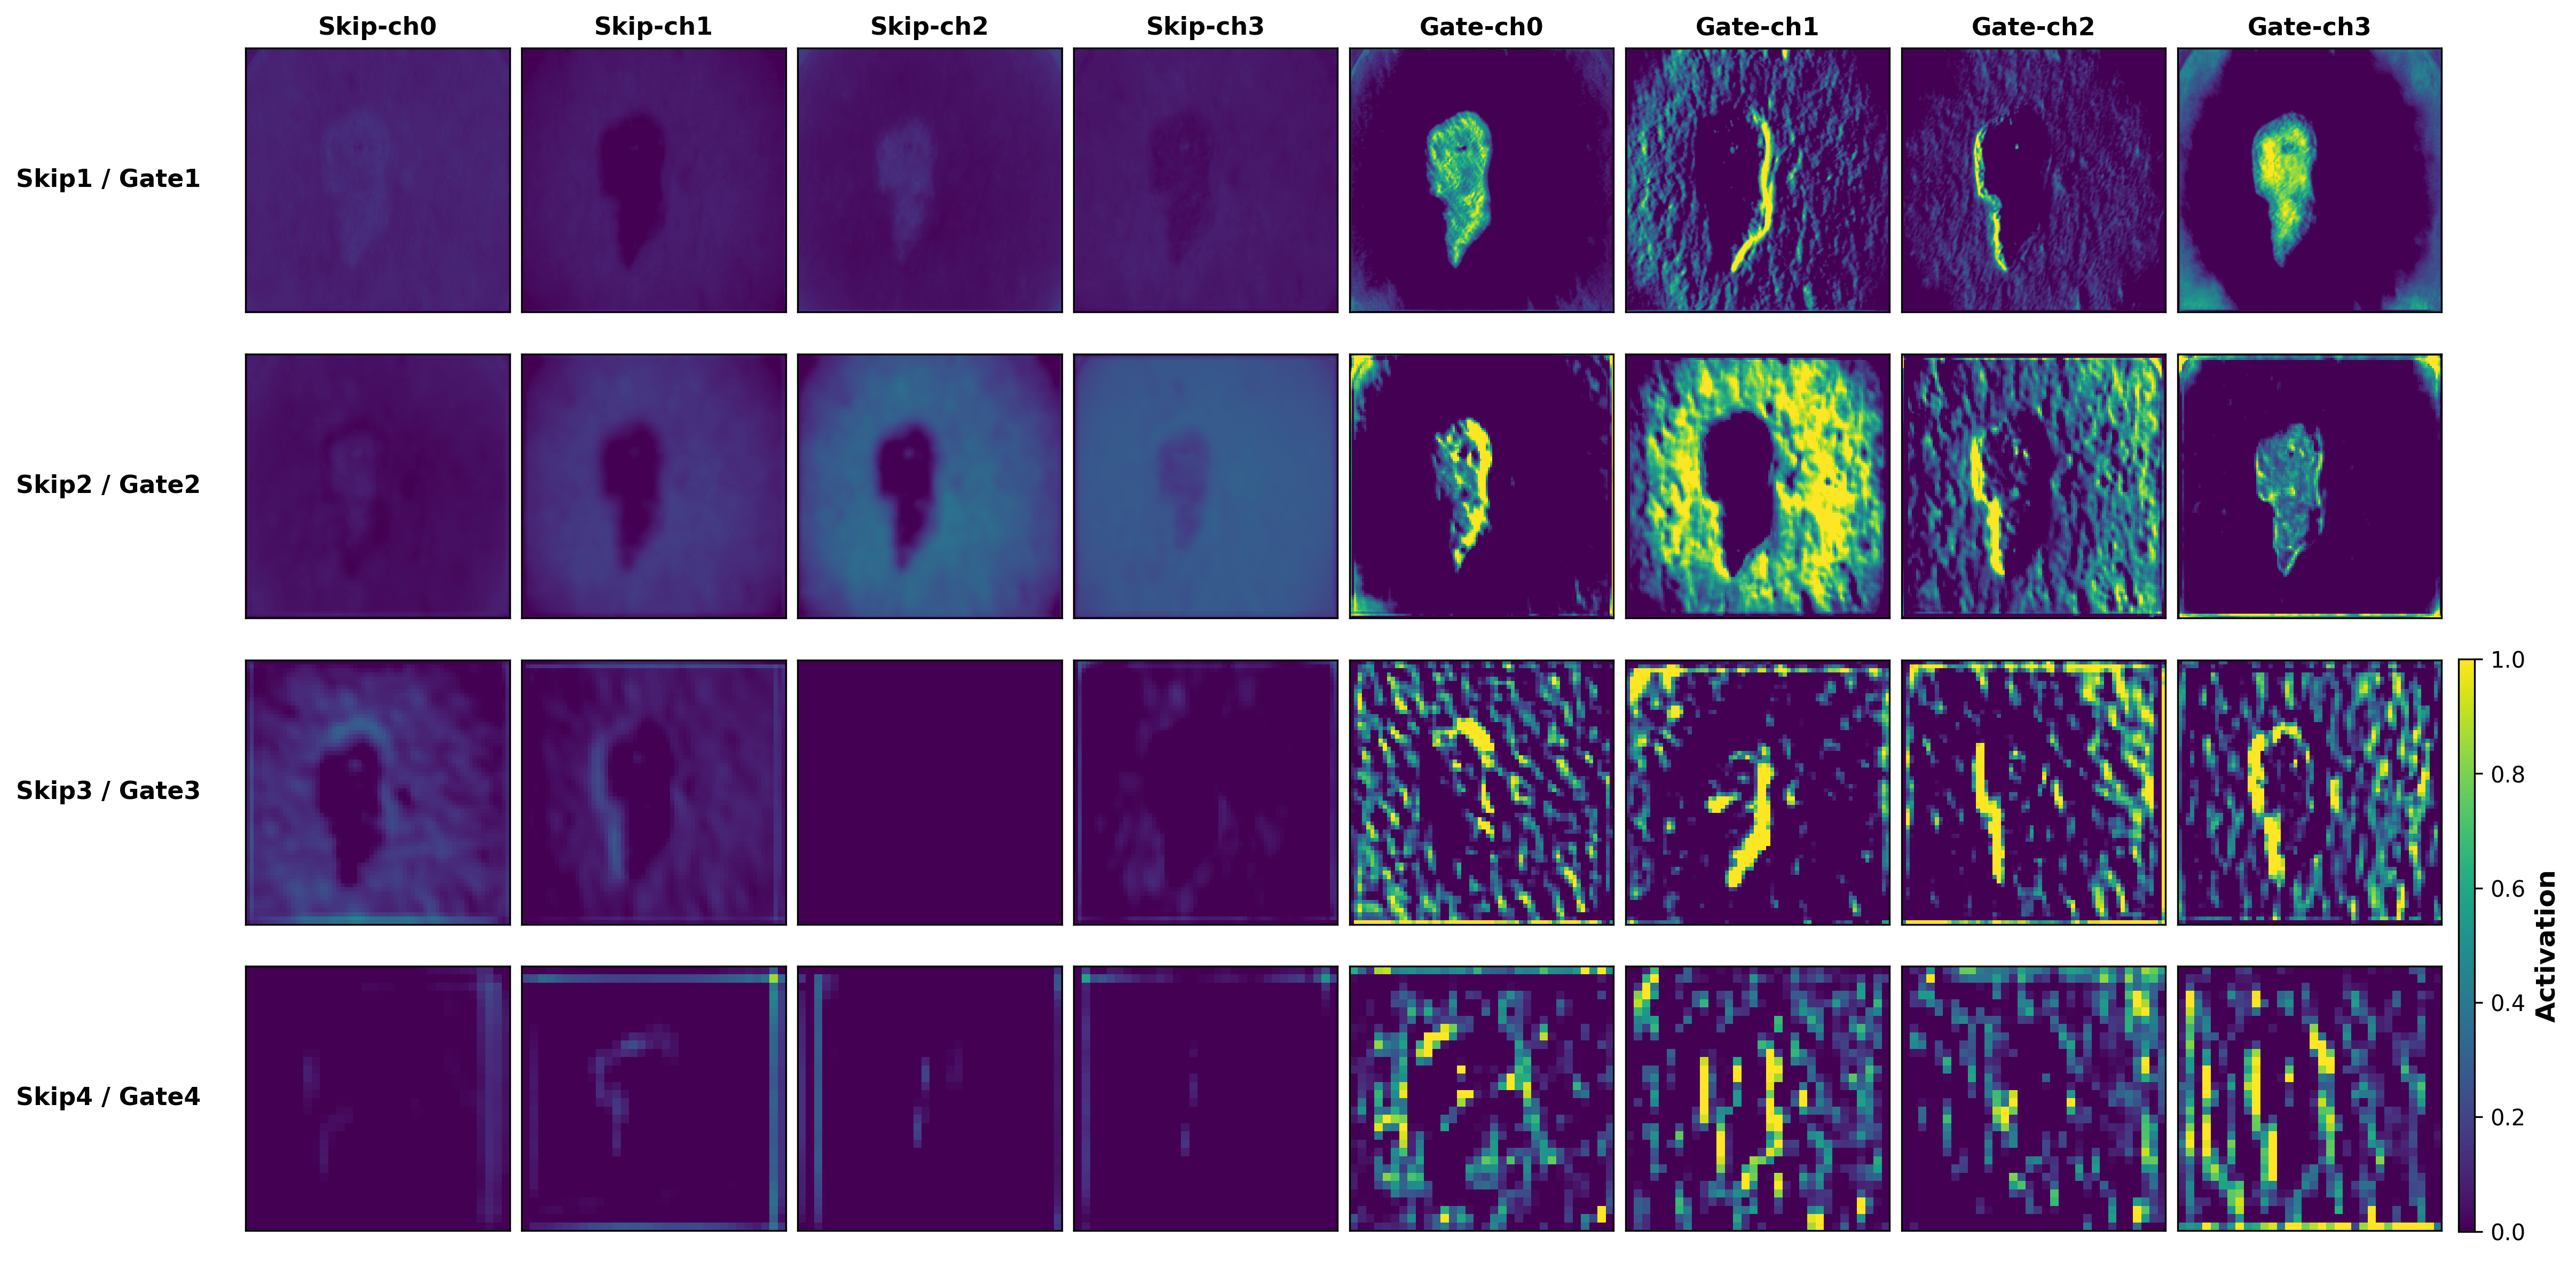
\includegraphics[width=\textwidth]{fig/unet_vs_attunet_feature_compare.png}
    \caption{基准 U-Net (左) 与 Attention U-Net (右) 在四级跳跃连接路径上的特征响应对比}
    \label{fig:skip_vs_gate_vis}
\end{figure}

经过对比之后可以看出注意力门起到了增益和抑制双向调制的作用:一方面降低了噪声,另一方面放大了关键特征,在解码阶段提供了更清晰的边界信息。

在Skip1以及Skip2当中,原始特征在几乎整幅图像上都呈现出弱激活的状态,背景纹理和病灶边界很难进行区分,然而在Gate1、Gate2里,大量的背景像素被压制到了0至0.2的低激活区域,仅仅是在病灶主体及其边缘位置保留了响应,这也就说明注意力门在最早的层面就已经将无用的纹理过滤掉了。同时,随着网络不断加深,原始的跳跃特征已经极其不明显,但是Gate3、Gate4的高亮区域收缩并且对齐在了病灶外轮廓上,形成了清晰的连贯带,由此可看出,门控权重抑制了背景,还在深层强化了对判别性边界的响应。

上述可视化的结果与前文中对注意力门原理的描述一致,也为后续消融实验结果(见第 5.2.5 节)提供了直观的佐证:较基准模型,引入注意力机制的U-Net模型在验证集 Recall 和 Dice 均显著提高,而 Precision 仅出现轻微波动。这说明注意力门能够在跳跃连接中对高分辨率特征进行“像素级甄别”,在最大限度保留判别性信息的同时,有效压制背景噪声,从源头减少漏检而不过度引入误检。

\subsection{损失函数的改进设计}

在损失函数的设计上,改进的U-Net模型采用Dice Loss和Cross-Entropy Loss的混合损失函数,即以相等权重线性叠加Dice损失与像素级交叉熵(CE)损失,以充分兼顾类别不平衡下的区域重叠度优化与梯度稳定性。设网络输出的类别概率图(像素总数为$N$)为:$ P=\left\{p_{i}\right\}_{i=1}^{N} $,真实分割掩膜为$ G=\left\{g_{i}\right\}_{i=1}^{N} $,其中$ p_{i} \in[0,1], g_{i} \in\{0,1\}$分别是像素$i$的前景概率和真实标签。则:

\begin{equation}
    \mathcal{L}_{\text {Dice }}=1-\frac{2 \sum_{i=1}^{N} p_{i} g_{i}}{\sum_{i=1}^{N} p_{i}+\sum_{i=1}^{N} g_{i}+\varepsilon}
\end{equation}

\begin{equation}
    \mathcal{L}_{\mathrm{CE}}=-\frac{1}{N} \sum_{i=1}^{N}\left[g_{i} \ln \left(p_{i}\right)+\left(1-g_{i}\right) \ln \left(1-p_{i}\right)\right]
\end{equation}

\begin{equation}
    \mathcal{L}_{\text {mix }}=0.5 \mathcal{L}_{\text {Dice }}+0.5 \mathcal{L}_{\mathrm{CE}}
\end{equation}

其中$ \varepsilon=10^{-6} $用于数值平滑以防零分母。Dice项直接对预测与标注的重叠区域进行归一化度量,能在小体积病灶场景下显著提升召回;交叉熵项则提供像素级对数似然的密集监督,改善早期训练阶段梯度稀疏、收敛震荡等问题。

\subsection{训练策略的改进设计}

根据Marire-Hein等人\cite{maier-hein2018a}的统计,大量医学图像挑战赛的训练集大小平均集中在100\~400之间。对于本研究使用的三个数据集:ISIC、LiTS和BraTS,其情况和特点已在3.1节进行l了详细阐述。从数据集规模看,三个数据集在样本数量上均已达到医学图像语义分割的中等规模。然而对于医学图像语义分割任务,在医学图像的目标结构和背景环境都较为一致的情况下,模型的训练容易学习到固定的像素分布模式,而非像素语义概念,进而使得模型对输入数据的轻微旋转、形变和灰度偏移变得十分敏感。

基于上诉分析,单纯的依赖原始样本不足以支撑有效的特征学习,在这种情况下,采用数据增强策略是提升模型性能和稳定性的关键。在对多项医学图像分割竞赛模型的系统分析中,Maier-Hein等人\cite{maier-hein2018a}指出,几乎所有方法都采用了数据增强策略,尤其是在病例数量在200+左右时。此外,Isensee等人在提出nnU-Net网络时也明确强调\cite{isensee2021},即使在中等数据规模的数据集上,不做数据增强也会严重影响模型验证集的性能。

因此,本研究在改进的U-Net模型设计中引入了包括随机旋转、水平垂直翻转以及弹性形变的数据增强训练策略,以帮助模型提升对于图像取向、灰度变化和形态扰动的鲁棒性和学习有泛化能力的语义特征表示。